\documentclass{article}

\usepackage{amsmath}
\usepackage{amsfonts}
\usepackage{amssymb}
\usepackage[utf8]{inputenc}
\usepackage{graphicx}
\usepackage[margin=0.5in]{geometry}
\usepackage{csvsimple}

\usepackage{listings}

\title{Assignment 2}
\author{Miguel A. Gomez B.}

\begin{document}
	\maketitle
\paragraph{} \textit{(50 points)} Many problems in science and mathematics involve iterations. In dynamics, the process that is repeated is the application of a function. To iterate a function means to evaluate the function over and over, using the output of the previous application as the input for the next. Matematically, this is the process of repeatedly composing the function with itself. Given $x_0 \in \mathbb{R}$ we define the orbit of $x_0$ under $F$ to be the sequence of points $x_0, x_1 = F(x_0),\dots, x_n = F^n(x_0)$\footnote{Note that $F^n(x)$ does not mean raise $F(x)$ to the $n$th power (an operation we will never use). It is the $n$th iterate of $F$ evaluated at $x$.}. The point $x_0$ is called the \textit{seed} of the orbit.
\paragraph{}With this in mind, let us play with the following function:
\[ 
	F(x) = 
	\begin{cases} 
		2x & 0 \leq x < \frac{1}{2} \\
		2x - 1 & \frac{1}{2} \leq x < 1
	\end{cases}
\]
\paragraph{} The code of this point can be looked at \textit{RunMeInPython.py}.
\paragraph{1} Choose 5 different initial seeds that should be in the interval $[1,0)$ and for each one compute the first $100$ points on the corresponding orbit. Record the results by listing the initial seed together with what happened to the orbit.
\begin{center}
	\csvautotabular{some_results}
\end{center}
\paragraph{} the complete results can be found on the file \textit{results}.
\paragraph{(a)}\textit{(20 points)} Plot the results of the two cases in a plane $x_i$ vs $x_{i+1}$.
\begin{center}
	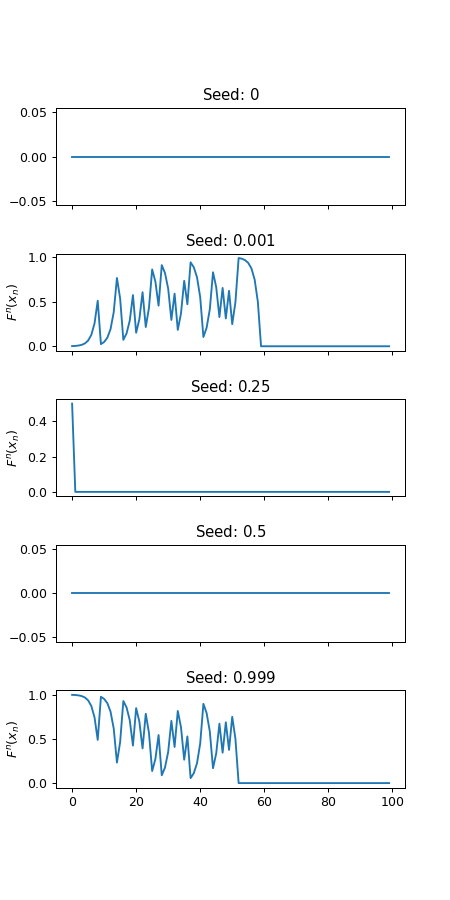
\includegraphics[width=0.5\textwidth]{plots_v2}
\end{center}
\paragraph{(b)}\textit{(10 points)}Do they have a visible pattern? Do all (or almost all) orbits behave in the same way?.
\paragraph{} As it was expected with the exact values of $0$ and $0.5$ nothing interesting happens, the orbit moves from the seed to zero, but, with values closer to $0$ and $1$ (which are limits of the intervals on which the function is defined), the orbit shifts in a visible pattern from increase to decrease to finally go to $0$. But actually different patterns arise with different values on the seed.
\begin{center}
	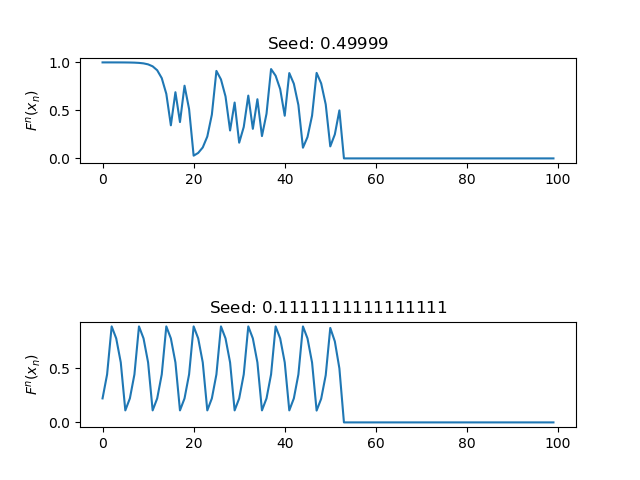
\includegraphics[width=0.7\textwidth]{plot_2.png}
\end{center}
So for different seed values we have different behavior on the orbits.
\newpage
\paragraph{(c)}\textit{(20 points)} For the same two discussed cases, instead of treating the seeds a floating point numbers, use \textit{SymPy} to do the exact rational arithmetic. Do the same for the seed $x_0=\frac{1}{9}$. What do you find for these three cases? Does the computer lie?
\begin{center}
	\csvautotabular{some_weird_results}
\end{center}
\paragraph{} The complete results can be found on the file \textit{weird\_results}, the code file used to generate this values is \textit{orbits\_sympy.py}.
\paragraph{} The data shows a diferent behavior, also notice that \textit{seed6} corresponds to the seed $\frac{1}{9}$. lets look at the graph and analyze the results.
\begin{center}
	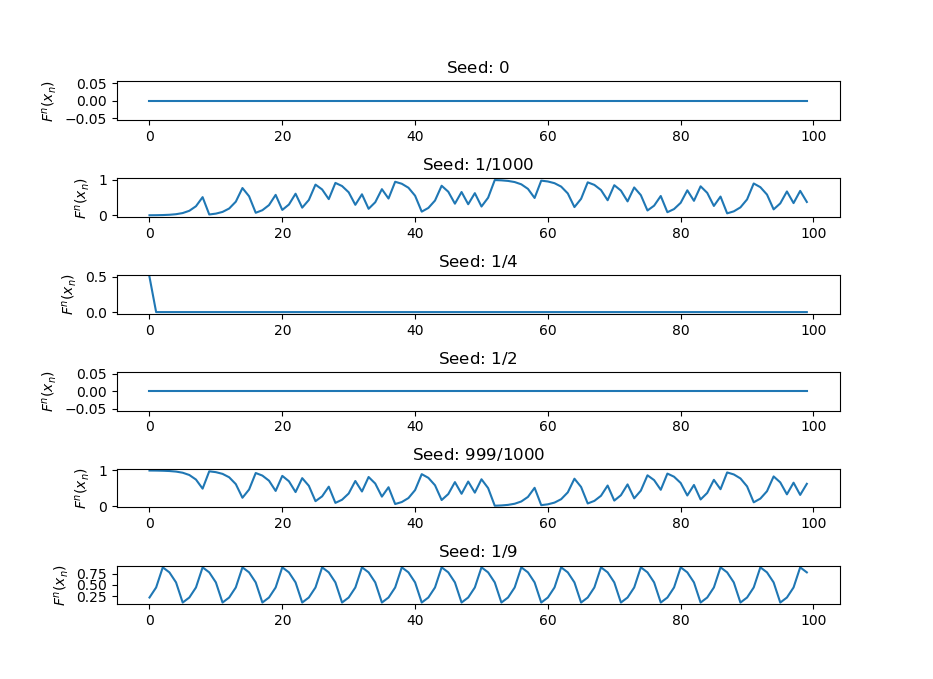
\includegraphics[width=0.7\textwidth]{plots_weird.png}
\end{center}
\begin{center}
	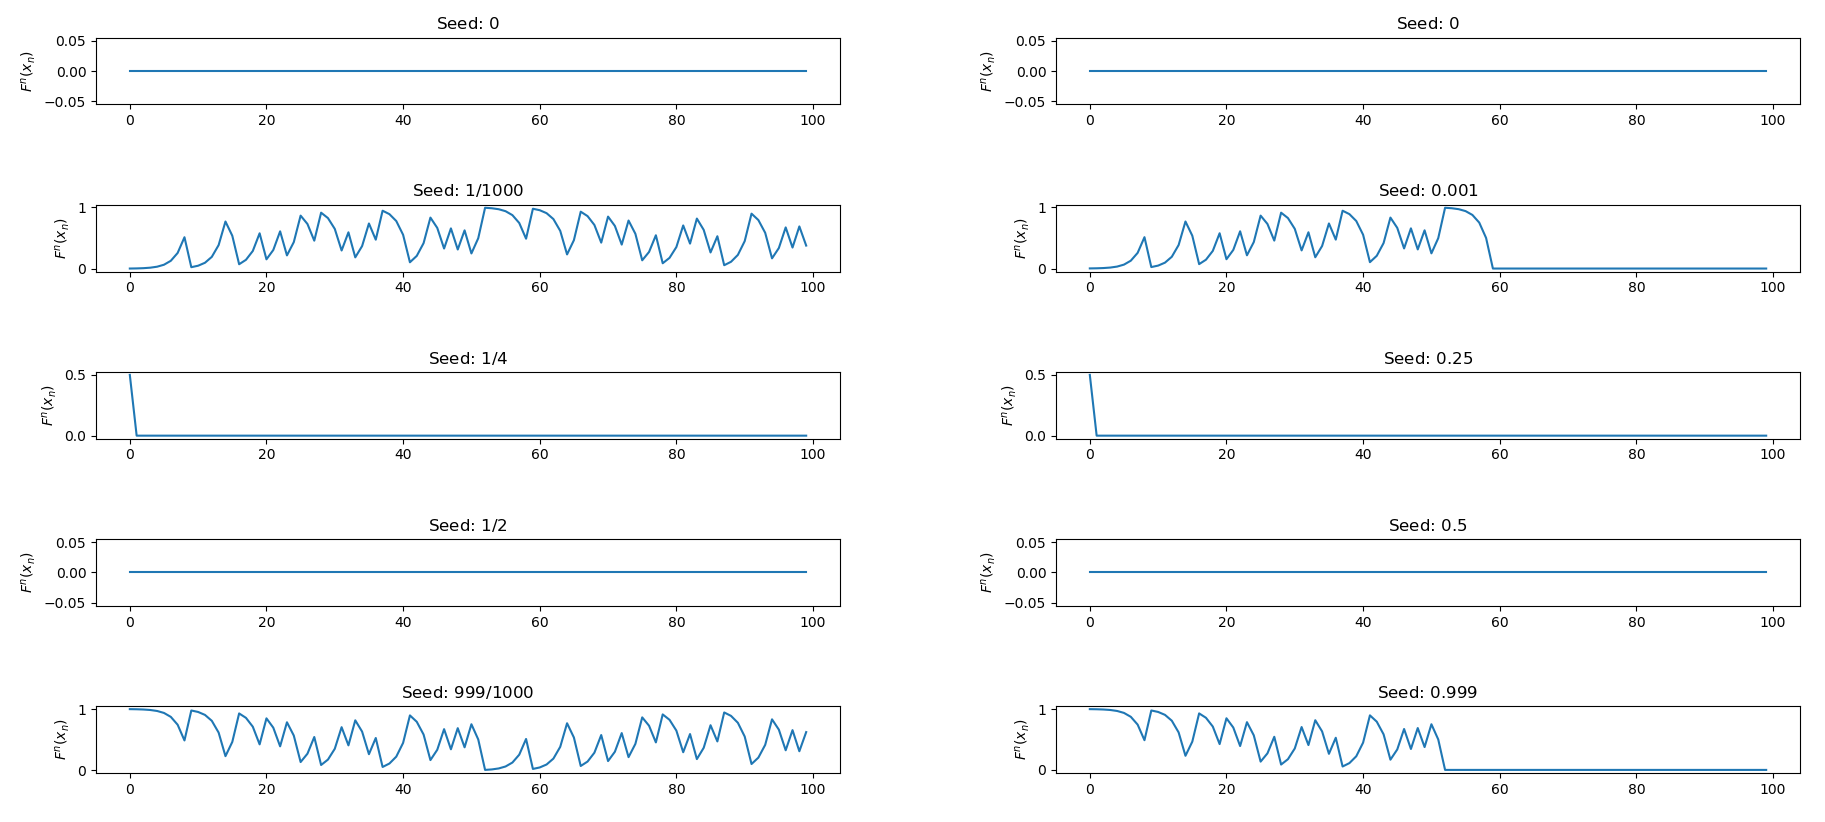
\includegraphics[width=\textwidth]{vs.png}
\end{center}
\paragraph{}With the seeds $0$ and $0.5$, there is no difference but on the seeds $\frac{1}{1000} = 0.001$ and $\frac{999}{1000} = 0.999$, visually we can see that there is no difference up to some point, The data shows an slightly difference at some point of the computation:
\begin{center}
	\csvautotabular{some_differences}
\end{center}
\paragraph{}The symbolic solution it is a better approximation, the same happens with the seed $\frac{1}{9}$:
\begin{center}
	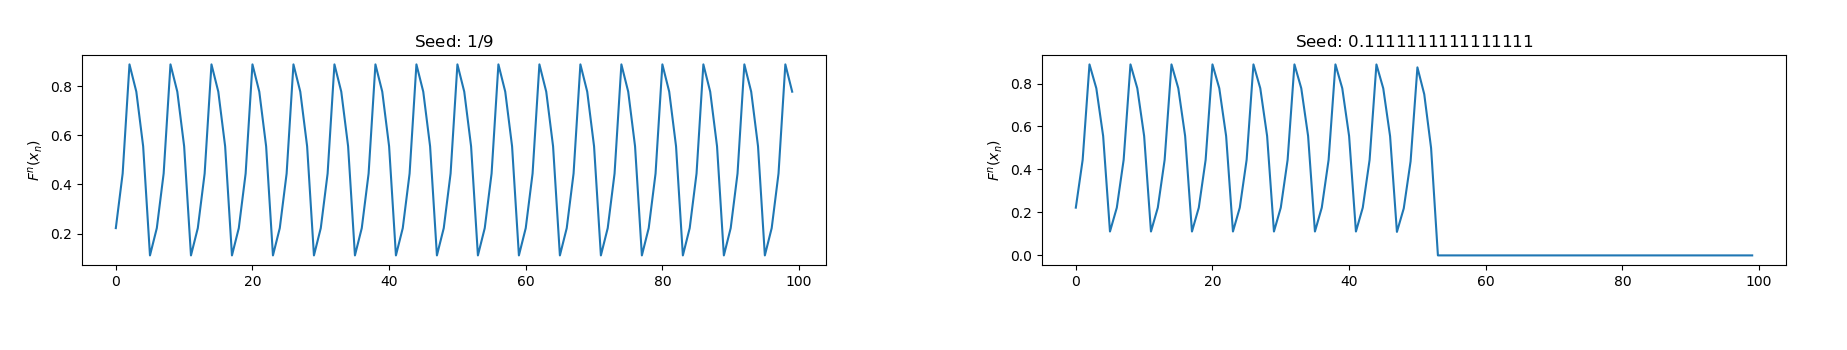
\includegraphics[width=0.7\textwidth]{9.png}
\end{center}
\begin{center}
	\csvautotabular{9_some_differences}
\end{center}
We can now explain why this happens, and it is related to the approximation that the numeric solution does, notice that $\frac{1}{9} \approx 0.11111...$ but the computer has limited resources, so by convention some approximation to this number is performed when the numeric solution is executed. By contrast, the symbolic computation does not seem to use the same logic, we can conclude that the behavior is in reality given by the way the computer deals with the computation, the technical name for this approximation is related to the value of the EPS constant or machine epsilon, this constant determines the upper bound on the relative error due to a float point number arithmetic. On my machine this value corresponds to $2.220446049250313e-16$ for the float data type, at some point the operation in the program exceeded this constant propagating rounding errors that got bigger at later iterations.
\end{document}